% ----------------------------------------------------------------
%       Speech Signal Processing Toolkit (SPTK): version 3.0
%                      SPTK Working Group
% 
%                Department of Computer Science
%                Nagoya Institute of Technology
%                             and
%   Interdisciplinary Graduate School of Science and Engineering
%                Tokyo Institute of Technology
%                   Copyright (c) 1984-2000
%                     All Rights Reserved.
% 
% Permission is hereby granted, free of charge, to use and
% distribute this software and its documentation without
% restriction, including without limitation the rights to use,
% copy, modify, merge, publish, distribute, sublicense, and/or
% sell copies of this work, and to permit persons to whom this
% work is furnished to do so, subject to the following conditions:
% 
%   1. The code must retain the above copyright notice, this list
%      of conditions and the following disclaimer.
% 
%   2. Any modifications must be clearly marked as such.
%                                                                        
% NAGOYA INSTITUTE OF TECHNOLOGY, TOKYO INSITITUTE OF TECHNOLOGY,
% SPTK WORKING GROUP, AND THE CONTRIBUTORS TO THIS WORK DISCLAIM
% ALL WARRANTIES WITH REGARD TO THIS SOFTWARE, INCLUDING ALL
% IMPLIED WARRANTIES OF MERCHANTABILITY AND FITNESS, IN NO EVENT
% SHALL NAGOYA INSTITUTE OF TECHNOLOGY, TOKYO INSITITUTE OF
% TECHNOLOGY, SPTK WORKING GROUP, NOR THE CONTRIBUTORS BE LIABLE
% FOR ANY SPECIAL, INDIRECT OR CONSEQUENTIAL DAMAGES OR ANY
% DAMAGES WHATSOEVER RESULTING FROM LOSS OF USE, DATA OR PROFITS,
% WHETHER IN AN ACTION OF CONTRACT, NEGLIGENCE OR OTHER TORTIOUS
% ACTION, ARISING OUT OF OR IN CONNECTION WITH THE USE OR
% PERFORMANCE OF THIS SOFTWARE.
% ----------------------------------------------------------------
%
\name{grlogsp}{draw a running log spectrum graph}{plotting graphs}

\begin{synopsis}
\item[grlogsp] [ --t ] [ --O $O$ ] [ --x $X$ ] [ --y $ymin$ ] [ --yy $YY$ ]
	       [ --yo $YO$ ] [ --p $P$ ] 
\item[\ ~~~~~~~~] [ --ln $LN$ ] [ --s $S$ ] [ --e $E$ ] [ --n $N$ ] [ --l $L$ ] 
\item[\ ~~~~~~~~] [ --c $comment1$ ] [ --c2 $comment2$ ] [ --c3 $comment3$ ]
		  [ {\em infile} ]
\end{synopsis}

\begin{qsection}{DESCRIPTION}
{\em grlogsp} converts a sequence of float-format log spectra 
from {\em infile} (or standard input) 
to a running spectrum plot in FP5301 plot format,
sending the result to standard output. 
The output can viewed with ``xgr''.

{\em grlogsp} is implemented as a shell script 
that uses the ``fig'' and ``fdrw'' commands.
\end{qsection}

\begin{options}
	\argm{t}{}{transpose x and y axes}{FALSE}
	\argm{O}{O}{origin of graph\\
		      \begin{minipage}{4cm}
		      \begin{tabular}{ccc}
			1 & ( 25,$YO$) & [mm] \\
			2 & ( 60,$YO$) & [mm] \\
			3 & ( 95,$YO$) & [mm] \\
			4 & (130,$YO$) & [mm] \\
			5 & (165,$YO$) & [mm]
		      \end{tabular}\\\hspace*{\fill}
		      \end{minipage}
		      \begin{minipage}{4cm}
			    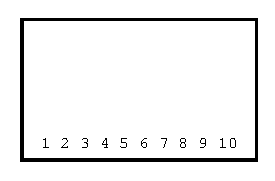
\includegraphics{fig/grlogsp-on.eps}
		      \end{minipage}\\\hspace*{\fill}\\
		    $(YO + 100 , X)$ [mm] if -t is specified.}{1}
	\argm{x}{X}{ $x$ scale\\
		       \begin{tabular}{cl}
			1 & normalized frequency($0 \sim 0.5$) \\
			2 & normalized frequency($0 \sim \pi$) \\
			4 & frequency($0 \sim 4$kHz) \\
			5 & frequency($0 \sim 5$kHz) \\
			8 & frequency($0 \sim 8$kHz) \\
			10 & frequency($0 \sim 10$kHz) \\
		       \end{tabular}\\\hspace*{\fill}}{1}
	\argm{y}{ymin}{ $y$ minimum}{-100}
	\argm{yy}{YY}{ $y$ scale [dB/10mm]}{100}
	\argm{yo}{YO}{ $y$ offset}{30}
	\argm{p}{p}{type of pen ($1 \sim 10$)}{2}
	\argm{ln}{LN}{style of line($0 \sim 5$).
                      please refer to fig command section.}{1}
	\argm{s}{S}{start frame number}{0}
	\argm{e}{E}{end frame number}{EOF}
	\argm{n}{N}{number of frame}{EOF}
	\argm{l}{L}{frame length.
                    Actually $\frac{L}{2}$ data are plotted.}{256}
	\argm{c, c2, c3}{\mbox{\em comment} 1 \sim 3}%
                        {comment for the graph}{N/A}
	\desc[1ex]{Usually, the options below do not need to be assigned.}
	\argm{W}{W}{width of the graph($\times 100$mm)}{0.25}
	\argm{H}{H}{height of the graph($\times 100$mm)}{1.5}
	\argm{z}{Z}{This option is used when data is written
                    recursively in the $y$ axis. the distance between
                    two graphs in the $y$ axis are given by $Z$.}{1}
	\argm{o}{xo \; yo}{origin of the graph.
                      if -o option exists, -O is not effective.}{95 30}
	\argm{g}{G}{type of frame of the graph($0 \sim 2$).
                    please refer to ``fig'' command section.}{2}
	\argm{cy}{cy}{first comment position}{-8}
	\argm{cy2}{cy2}{second comment position}{-14}
	\argm{cy3}{cy3}{third comment position}{-20}
	\argm{cs}{cs}{font size of the comments}{1}
	\argm{f}{f}{additional data file for fig}{NULL}
\end{options}

\begin{qsection}{EXAMPLE}
In this example, the magnitude of log spectrum is evaluated from
data in {\em data.f} file in float format, and the graph
with the running spectrum is sent in Postscript format to {\em data.ps}
file:
\begin{quote}
 \verb!frame < data.f | window |\! \\
 \verb!uels -m 15 | c2sp -m 15 |\! \\
 \verb!grlogsp | psgr > data.ps!
 \end{quote}
\end{qsection}

\begin{qsection}{SEE ALSO}
 fig, fdrw, xgr, psgr, glogsp, gwave
\end{qsection}
